
%%%%%%%%%%%%%%%%%%%%%%% file typeinst.tex %%%%%%%%%%%%%%%%%%%%%%%%%
%
% This is the LaTeX source for the instructions to authors using
% the LaTeX document class 'llncs.cls' for contributions to
% the Lecture Notes in Computer Sciences series.
% http://www.springer.com/lncs       Springer Heidelberg 2006/05/04
%
% It may be used as a template for your own input - copy it
% to a new file with a new name and use it as the basis
% for your article.
%
% NB: the document class 'llncs' has its own and detailed documentation, see
% ftp://ftp.springer.de/data/pubftp/pub/tex/latex/llncs/latex2e/llncsdoc.pdf
%
%%%%%%%%%%%%%%%%%%%%%%%%%%%%%%%%%%%%%%%%%%%%%%%%%%%%%%%%%%%%%%%%%%%


\documentclass[runningheads,a4paper]{llncs}

\usepackage{amssymb}
\setcounter{tocdepth}{3}
\usepackage{graphicx}

\usepackage{url}
\urldef{\mailsa}\path|{alfred.hofmann, ursula.barth, ingrid.haas, frank.holzwarth,|
\urldef{\mailsb}\path|anna.kramer, leonie.kunz, christine.reiss, nicole.sator,|
\urldef{\mailsc}\path|erika.siebert-cole, peter.strasser, lncs}@springer.com|
\newcommand{\keywords}[1]{\par\addvspace\baselineskip
\noindent\keywordname\enspace\ignorespaces#1}

\begin{document}

\mainmatter  % start of an individual contribution

% first the title is needed
\title{Versioning for Software as a Service in the context of Multi-Tenancy}

% a short form should be given in case it is too long for the running head

% the name(s) of the author(s) follow(s) next
%
% NB: Chinese authors should write their first names(s) in front of
% their surnames. This ensures that the names appear correctly in
% the running heads and the author index.
%
\author{Maximilian Schneider \and Johan Uhle}
%
% (feature abused for this document to repeat the title also on left hand pages)

% the affiliations are given next; don't give your e-mail address
% unless you accept that it will be published
\institute{University of Potsdam, Hasso-Plattner-Institute\\
Prof.-Dr.-Helmert-Str. 2-3, 14482 Potsdam, Germany\\
\path|{maximilian.schneider, johan.uhle}@student.hpi.uni-potsdam.de|}

%
% NB: a more complex sample for affiliations and the mapping to the
% corresponding authors can be found in the file "llncs.dem"
% (search for the string "\mainmatter" where a contribution starts).
% "llncs.dem" accompanies the document class "llncs.cls".
%

\toctitle{Lecture Notes in Computer Science}
\tocauthor{Authors' Instructions}
\maketitle


\begin{abstract}
TODO

How to provide different versions of a SaaS to multiple tenants at the same time?

\keywords{TODO}
\end{abstract}

\section{Introduction}

Boom \cite{Bezemer2010}

You are strongly encouraged to use \LaTeXe{} for the
preparation of your camera-ready manuscript together with the
corresponding Springer class file \verb+llncs.cls+. Only if you use
\LaTeXe{} can hyperlinks be generated in the online version
of your manuscript.

The \LaTeX{} source of this instruction file for \LaTeX{} users may be
used as a template. This is
located in the ``authors'' subdirectory in
\url{ftp://ftp.springer.de/pub/tex/latex/llncs/latex2e/instruct/} and
entitled \texttt{typeinst.tex}. There is a separate package for Word
users. Kindly send the final and checked source
and PDF files of your paper to the Contact Volume Editor. This is
usually one of the organizers of the conference. You should make sure
that the \LaTeX{} and the PDF files are identical and correct and that
only one version of your paper is sent. It is not possible to update
files at a later stage. Please note that we do not need the printed
paper.

We would like to draw your attention to the fact that it is not possible
to modify a paper in any way, once it has been published. This applies
to both the printed book and the online version of the publication.
Every detail, including the order of the names of the authors, should
be checked before the paper is sent to the Volume Editors.

\subsection{Checking the PDF File}

Kindly assure that the Contact Volume Editor is given the name and email
address of the contact author for your paper. The Contact Volume Editor
uses these details to compile a list for our production department at
SPS in India. Once the files have been worked upon, SPS sends a copy of
the final pdf of each paper to its contact author. The contact author is
asked to check through the final pdf to make sure that no errors have
crept in during the transfer or preparation of the files. This should
not be seen as an opportunity to update or copyedit the papers, which is
not possible due to time constraints. Only errors introduced during the
preparation of the files will be corrected.

This round of checking takes place about two weeks after the files have
been sent to the Editorial by the Contact Volume Editor, i.e., roughly
seven weeks before the start of the conference for conference
proceedings, or seven weeks before the volume leaves the printer's, for
post-proceedings. If SPS does not receive a reply from a particular
contact author, within the timeframe given, then it is presumed that the
author has found no errors in the paper. The tight publication schedule
of LNCS does not allow SPS to send reminders or search for alternative
email addresses on the Internet.

In some cases, it is the Contact Volume Editor that checks all the final
pdfs. In such cases, the authors are not involved in the checking phase.

\subsection{Additional Information Required by the Volume Editor}

If you have more than one surname, please make sure that the Volume Editor
knows how you are to be listed in the author index.

\subsection{Copyright Forms}

The copyright form may be downloaded from the ``For Authors"
(Information for LNCS Authors) section of the LNCS Website:
\texttt{www.springer.com/lncs}. Please send your signed copyright form
to the Contact Volume Editor, either as a scanned pdf or by fax or by
courier. One author may sign on behalf of all of the other authors of a
particular paper. Digital signatures are acceptable.

\section{Terminology (Max)}
\label{sec:terminology}

\subsection{Multi-Tenancy}

Software as a Service products are usually built for multi-user usage. In Multi-tenancy, these users belong to one tenant and need to be isolated from other tenants' users. Each tenant has hereby access to an isolated multi-user system \cite{Chong2006a}. To sell the products to a wide variety of tenants the software is usually heavily customizable and secured by Service Level Agreements~\cite{Bezemer2010}.

Multi-Tenancy itself should not be confused with multi-tenancy architecture which differs from multi-instance architecture by servicing multiple tenants from a single instance of the software~\cite{Shao2011} in contrast to providing a dedicated instance of the software to each tenant.

%What is multi tenancy? How does it relate to multi user?
  %multi-user is a subset of multi-tenant
  %every tenant is a multi-user system in itself
  %Multi-tenant =  Multi-User + SLA + Heavily customizable [DELFT]
\subsection{Version}

Considering software versioning two different definitions exists. One is the \emph{product version}, which identifies a certain stage of the software in a release lifecycle. The other is a \emph{code revision}, which is managed by a version control system as part of software configuration management \cite{swebook}.

% coupling: It might be belong to an actual product version
As the latter definition in contrast to the former is mainly dealing with changes to the source code, differences in code revisions might not be distinguishable by the users, whereas product versions are inherently visible to the users. In this report we are concerned with product versions and do not further discuss code revisions.

%(Frontend:UI/Backend:Busisness Logix/DB)
  %- // how can we provide a versioning for all these layers with minimal cost. where the tenant can choose.
  %- // how can we make sure that everything is in sync and consistent
  %- granularity of versioning depends on how tight stack is coupled
  %- users interface with versioning in frontend (tenant or even user specific)
  %- backend/db is only versioned forward for whole tenant
  %- stick with product version instead of code revision
%- Configuration
  %- variables in database in shared table layout
%- Customization (int.)
  %- code / templating executed in the context of the saas provider
  %- huge changes
  %- // Eyad does not care about config/customization
  %- // predefined columns
  %- // Eyad doesn't care
  %- -> we handle just like configuration
  %Customization (internal)
  %Tenant-specific changes that run within the application context
  %Examples:
  %Templates, Custom DB fields, DSLs

%- Extension (ext.)
  %- // E column extension
  %- not focused on marketplace
  %- // truly external extensions are 2 much
  %- // Eyad doesn't care, we don't do
  %- -> we don't care
  %Extension (external)
  %Tenant-specific changes that run outside the application and interface with it over an API
  %Example:
  %Third-party add-ons in a marketplace
  %addon is in a way just a regular customer as it is truly external
  %we only have to consider customization in our architecture




\section{Related Work}
\label{sec:relatedwork}

- SaaS and Multi Tenancy
  - Economy of Scale
    - Development vs. Fixed Cost and Maintenance
    - Delft paper
- DB
  - A.Kemper "5-Schemas" -> MSDN 3 schemas
  - A.Kemper "Versioned Tables"

- Infrastructure
  - Salesforce as good Example
  - Delft no multi-instance
  - BPEL multi-instance used, though not wanted
- ...
  - Routing
  - Customization // how 2 either merge these approaches / try to map these approaches to something similiar or new on the application level
%!TEX root = ../report.tex

\section{Architecture}
\label{sec:architecture}

In this section we first clarify our assumptions about the \emph{application stack} of a SaaS. Then we explain the different architectures to implement  SaaS versioning.

One important assumption we make for versioning is, that each tenant and therefore also all users of a tenant use the same version at the same time. In practice this means that each tenant has a dedicated migration point in time at which they decide to switch the version. This switch affects all their users at the same time. Users aren't allowed to individually choose their version.

We furthermore assume that all requests to the SaaS are authenticated, thus there is always a user as well as a tenant and its version associated with each request.

\subsection{Application stack}
\label{sec:stack}

\begin{wrapfigure}{r}{0.28\textwidth}
  \begin{center}
    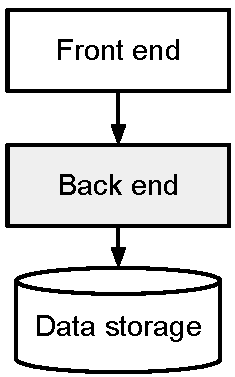
\includegraphics[width=0.28\textwidth]{stack.pdf}
    \caption{Simplified \protect\\ Application Stack}
    \vspace{-20pt}
    \label{fig:stack}
  \end{center}
\end{wrapfigure}


To understand the architecture better, we first want to look at the SaaS application stack as displayed in Figure~\ref{fig:stack}. We derived this stack from our experience with developing SaaS ourselves as well as stacks we have seen in related papers as depicted earlier in Section~\ref{sec:relatedwork}.

We assume a separation between the front end, back end and database layer. The \emph{front end layer} is mainly concerned with the user interface. In a SaaS it will usually be delivered to the user's browser within a HTTP request/response cycle. Another possible implementation for the front end layer is a webservice API that enables external applications (e.g. third-party or native applications) to communicate with the SaaS. We handle this more in-depth in Section~\ref{sec:sharedfrontend}. The \emph{back end layer} is concerned with the application and business logic. It handles requests of the front end layer and consequently communicates with the \emph{database layer}. To allow for horizontal scaling, the front end and back end layers are usually implemented stateless. All state is then kept in the database layer.

To focus our research, we omitted some details of the stack. We were not concerned with neither caching nor load balancing. Furthermore we omitted how user management is done, especially with regards to authentication.

\subsection{Multi-instance}

\begin{figure}
\vspace{-20pt}
\centering
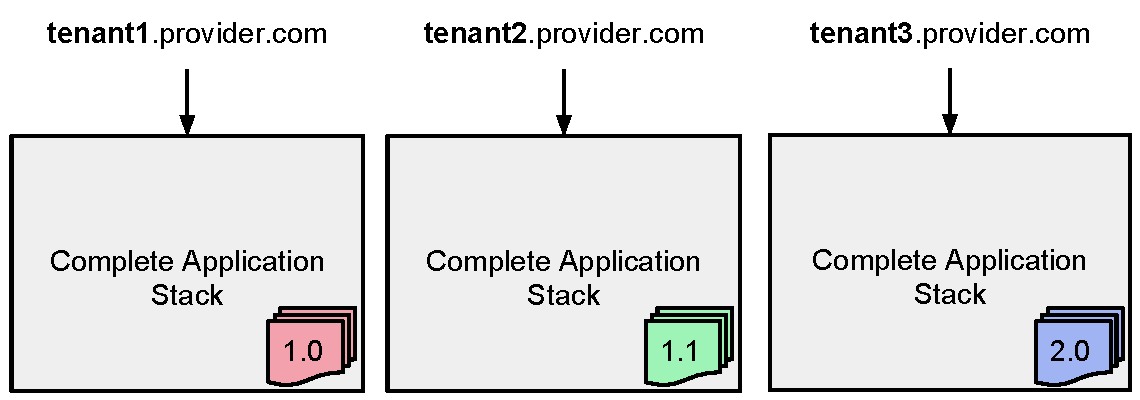
\includegraphics[width=\textwidth]{multiinstance.pdf}
\caption{Example for multi-instance with the respective software version for each tenant deployed on their instance}
\label{fig:multiinstance}
\vspace{-10pt}
\end{figure}

In a multi-instance architecture the whole application stack is deployed several times on dedicated resources. You can see an example in Figure~\ref{fig:multiinstance}. The multi-instance architecture serves the purpose of physical isolation of the tenants by provisioning resources for each tenant individually. Also it allows for developing a single-tenant application instead of building multi-tenancy awareness into the application.

This approach can also be used for versioning, where we see two variants:

\paragraph{Single instance per tenant} When every tenant has their own application stack instance running, these instances can be versioned by deploying the respective software version on the tenant's instance. See Figure~\ref{fig:multiinstance} for reference.
\paragraph{Single instance per version with multiple tenants} This is a hybrid approach where each instance has a specific version and the instances in turn can be hosts for multiple tenants by using the shared-instance mechanisms explained in the following section. See Figure~\ref{fig:multiinstance_versionstack} for reference.

\begin{figure}
\vspace{-15pt}
\centering
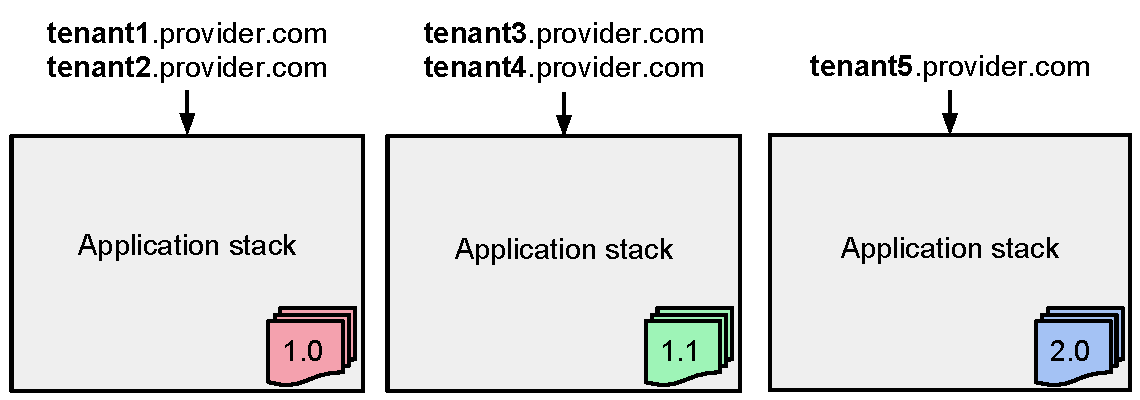
\includegraphics[width=\textwidth]{multiinstance_versionstack.pdf}
\caption{Example for a hybrid multi-instance approach which is multi-instance regarding the version, but shared-instance regarding the tenants}
\label{fig:multiinstance_versionstack}
\end{figure}

Using a multi-instance architecture has the benefits that the developers do not have to deal with issues concerning multi-tenancy in the application code. One of the drawbacks is the bad resource consolidation factor, thus if e.g. one tenant uses many resources but another uses none, the unused resources can't be allocated to the spiking tenant easily. Also the maintenance cost increases with the number of versions and tenants and there is no economy of scale working in favor of the SaaS provider then.

Versioning-wise the actual application stack is not version-aware and thus can be built without versioning as a concern. Instead versioning is handled on the deployment level. Migrations between versions might then need significant operations engineering effort.

\subsection{Shared-instance}

The shared-instance architecture consist of one software stack deployment that serves all tenants at the same time. This architecture is the one that is generally referred to when talking about multi-tenant SaaS applications, since it uses the economy of scale well due to its high consolidation factor \cite{Mietzner2009} \cite{Bezemer2010} \cite{Chong2006}.

To investigate versioning in the shared-instance architecture, we will individually inspect the layers of the application stack as outlined in the previous section, consisting of the front end, back end and database layer. For each layer we will outline how versioning can happen. We are closing this section with a look at how to migrate between versions.

\subsection{Shared-instance: Front-end layer}
\label{sec:sharedfrontend}

We split the \emph{front end layer} into two categories: a \emph{web application} running in the user's browser and an \emph{API consumer} e.g. running on the user's mobile phone.

\subsubsection{Web application} In web applications the user's browser is usually reloading the whole web page on each request, which mostly is triggered by an interaction of the user with the system\footnote{We assume that caching works transparently and perfectly as well as "One page applications" reloading their assets automatically ("hot code reload") in case something on the back end layer changes, as explained in \url{http://www.meteor.com/blog/2012/02/09/hot-code-pushes}}. Thus there is a tight coupling between the front end and the back end layer, from which we conclude that they are both versioned simultaneously. Since the front end software is delivered to the user's browser on each request, the versioning concern can be completely handled on the \emph{back end layer} as outlined in the next section.

\subsubsection{API consumer} To allow programmatic access to the SaaS functionality, SaaS providers usually implement a webservice. A common occurrence are HTTP APIs following the REST principles \cite{Fielding2000}. These APIs allow native applications (e.g. mobile phone applications) or other webservices to build on top of the SaaS. The SaaS and their API consumers are loosely coupled. They follow their own product cycles. In case of compatibility breaking changes in the SaaS API, the API consumers have to adapt to the changes and deploy a new version to their users. This might be hard to do e.g. because users might be reluctant to updates, delivery cycles might be too long or the API consumer developer might not have the resources to update their product. This leads us to the conclusion that SaaS APIs should be able to provide several versions at the same time. The API consumers choose which version of the API they want to use. There are many ways to handle versioning APIs and explaining them in-depth is out of the scope of this report. Examples are version numbers in the URL or \emph{HTTP Accept Header} of a request \cite{RFC2616}, or feature flags for the consumer application in the SaaS \cite{playbook2013} (as explained further in Section~\ref{sec:shared1n}).

  % Frontend API Versioning
  %   In URL:
  %     http://api.com/v1/resource.json?version=1
  %   Accept Header:
  %     Accept: application/json+v1
  %   Application Flag:

\subsection{Shared-instance: Back-end layer}
\label{sec:backend}

For versioning the back end layer we explore two variants: \emph{1:1} and \emph{1:n}.

\subsubsection{Shared-instance with 1:1 mapping}

\begin{figure}[h!]
\centering
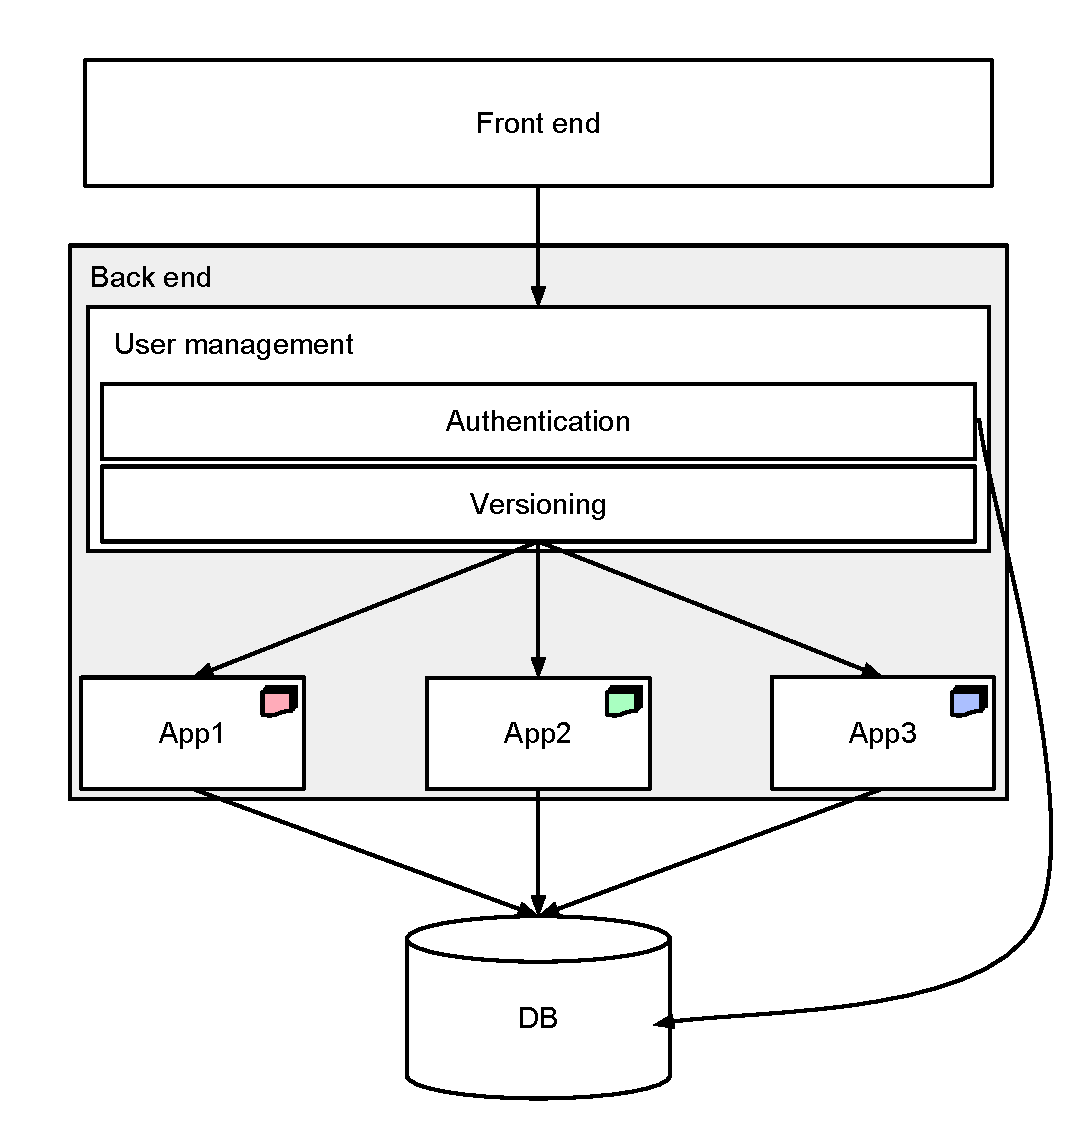
\includegraphics[width=\textwidth]{sharedinstance11.pdf}
\caption{Example for a shared-instance architecture with mapping each back end server to a code revision which in turn 1:1 maps to a product version}
\label{fig:sharedinstance11}
\end{figure}

The \emph{1:1 mapping} depicts that each product version is mapped to one code revision. Figure~\ref{fig:sharedinstance11} shows the architecture. Thus to support different product versions at the same time, the respective code revisions have to be deployed on different back end servers. On each request, the user management decides to which back end servers the request is routed, depending on the tenant the user belongs to.

The benefit of this approach is, that the versioning is happening outside of the application code, thus the code does not have to be version-aware. On the downsides, the consolidation factor of this approach is low, given that the load is split between non-consolidateable versions. This defecit increases with the increase of versions running in parallel. Furthermore this leads to a heterogeneous deployment which is more complex than a homogeneous deployment.  Also this can lead to problems like bugfixes, that if written once have to be merged and deployed into every running version. Also this approach needs an intelligent routing layer (in our example above the user management) which decides on which app server to map which request.

% a product ver = code rev
%
% Pro
% Versioning is external to application code
%
% Contra
% worse consolidation factor
% intelligent routing layer needed
% heterogeneous deployment
% forking of code base makes security patches difficult to apply

\subsubsection{Shared-instance with 1:n mapping}
\label{sec:shared1n}

\begin{figure}
\centering
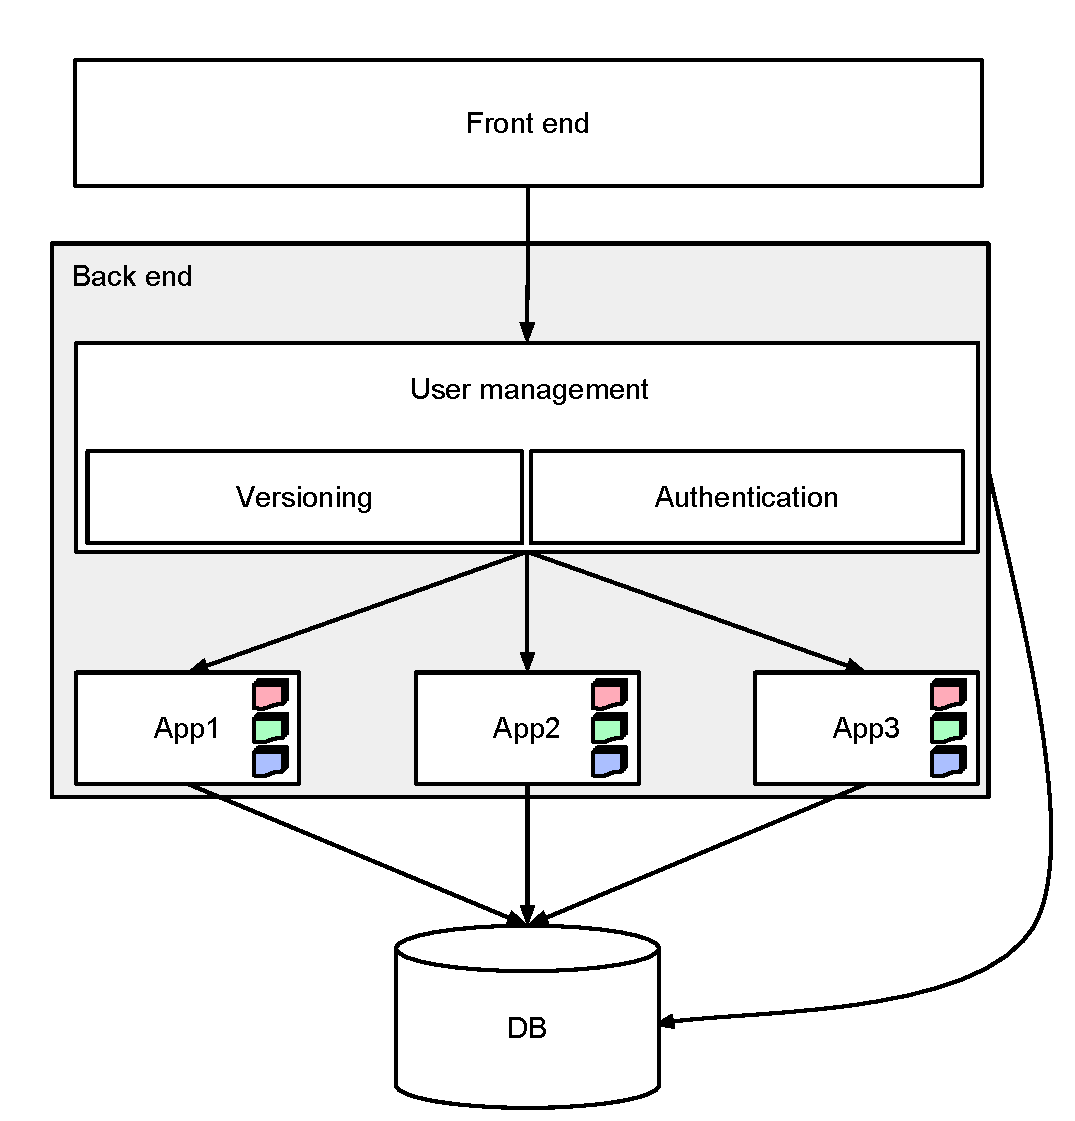
\includegraphics[width=\textwidth]{sharedinstance1n.pdf}
\caption{Example for a shared-instance architecture with mapping each back end server to a code revision which in turn can server several product versions}
\label{fig:sharedinstance1n}
\end{figure}

The \emph{1:n mapping} depicts that each code revision maps to all available \emph{n} product versions. As shown in Figure~\ref{fig:sharedinstance1n} each application server has the same code revision deployed and is therefore able to decide which product version to serve for each request. One way to implemented this is with feature flags. Listing~\ref{1ncode} shows a code example in Ruby. In the beginning of this section we assumed that every request has a user attached to it. Furthermore we assumed that all users of a tenant share the same version. This leads us to the conclusion, that the backend can determine the version for each incoming request.

\noindent\begin{minipage}{\textwidth}
  \lstset{language=Ruby, caption=Example code for \emph{1:n mapping} on an application server, label=1ncode}
  \begin{lstlisting}
    if user.has_version?("1.0")
      do_something()
    end

    if user.has_version?("1.1")
      do_something_a_bit_different()
    end
  \end{lstlisting}
\end{minipage}

The \emph{1:n mapping} approach has several benefits: The consolidation factor is high, since all app servers can serve all requests. The deployment is homogeneous over the app servers, thus making operations easier. Also it is possible to version more fine-grained, not only based on product versions but actually on feature level and even feature version. This opens up a tenant-feature matrix which allows versioning which is more flexible than the traditional linear versioning.
On the downside, the feature flags in the code increase code complexity, which might increase development time and increases the probability of bugs. Also the feature flags are spread over the code and removing them needs software development effort. Thus abandoning old versions is connected with extra cost.

% Pro
% good consolidation
% homogenous deployment
% more flexibility: fine grained feature selection
%
% Contra
% increased code complexity, might lead to more bugs
% high cost for abandoning old version to clean code base
%
%
% inside of code base are many version checks "if version == 1.4 ..."
% more flexibility in choosing version, maybe not choose version but choose only features

\subsection{Shared-instance: Database}
\label{sec:database}

The database is where state is kept. We assume that the database is a relational database, in that it keeps the data in tables with specified schemas to ensure the format and validity of the data.

In this section we will differentiate between two major cases regarding the database when versioning SaaS: \emph{Different versions share a compatible database schema} and \emph{different versions require different incompatible schemas}.

\subsubsection{Different versions share a compatible schema}
% TODO nice diagram?

When different versions share the same database schema, the database is actually agnostic to versioning. The changes of the versions happen in the other layers and thus never propagate down to the database. The same happens if changes are needed for one version, but the changes are compatible with the other versions. An example for this is the addition of new columns or tables. These can usually be ignored by versions that don't need these columns or tables, thus enabling compatibility with the changed schema.

\subsubsection{Different versions require different incompatible schemas}
% TODO nice diagram?

When schemas change between versions in an incompatible way, the database layer has to be versioned. Given that we assume we are dealing with a schema-enforcing database management systems (DBMS), the question is: How can schemas be versioned? How can a database support several schemas for the same data at the same time?

The problem is that current DBMS do always only support one schema at a time. In our research we did not find a DBMS that provides version-aware schemas. We investigate this option more in Section~\ref{sec:futurework}.

Since the database layer can not handle the versioning concern, the responsibility lies with the back end layer. Next we will investigate two approaches for that.

\paragraph{Different tables for each schema}

To store different schemas, a new database or table can be created for each version. An example with different tables can be seen in Listing~\ref{differenttablessql}. Each tenant is on a specific version, thus their data is stored in the corresponding table for their respective version.

\lstset{language=SQL, caption=sql, label=differenttablessql}
\begin{lstlisting}
  create table users_v1;
  create table users_v2;
  create table users_v3;
\end{lstlisting}

The problem with approach is that migrations between versions require moving the data of a whole tenant from the tables of one version to the tables of another version. This might include columns or even whole tables that were not changed between versions. This copying introduces a significant overhead which  current DBMS are not optimized for.

% TODO: Ich bin von den Pro/Cons nicht so richtig überzeugt
% Pro:
% Works well if not too many versions
%
% Con:
% Messy design if many versions

\paragraph{Pivot tables}

\begin{figure}
\centering
\includegraphics[width=\textwidth]{pivot.png}
\caption{Schema of pivot tables as shown in \cite{Yaish2011}}
\label{fig:pivot}
\end{figure}

Pivot tables as explained in \cite{Yaish2011} \cite{Aulbach2011} \cite{Weissman2009} follow the idea of not using a fixed schema in the database but keeping a flexible schema in the application. An example table layout can be seen in Figure~\ref{fig:pivot}. With pivot tables the DBMS is used more like a key-value store and in turn the application has to handle concerns that traditionally belonged to the DBMS, like query optimization or caching.

\subsubsection{Migration of data}

When a tenant decides to move to a new version and the new version requires a schema change, then the data of the tenant has to be migrated from the old to the new schema. Next we will describe two ways for running these migrations:

\paragraph{Batch-processing migration} The data is migrated in one go. Depending on the database management system, the schema changes and the amount of data, this process might take significant time. Depending on the algorithm used to execute the migration, the database and therefore the whole application might be completely unavailable or in read-only state for the tenant's users during the migration.
%TODO TO TALK ABOUT
\paragraph{On-the-fly migration} The data is migrated when it is requested or written. This could mean that clusters of data are migrated in batch (e.g. a user is migrated when she logs in) or are migrated row-by-row.

% version is chosen per tenant
% data migrations need time
% data migrations might need downtime
% on-the-fly migrations possible

\section{Future Work (Johan)}
\label{sec:futurework}

In our research we made two assumptions that simplified our setup but could yield interesting future work:

\paragraph{Switching versions per user} In Section~\ref{sec:stack} we assumed that a tenant chooses the version for all their users at the same time. Future research should investigate how versioning on the user-level could be implemented, especially when schema changes are involved.

\paragraph{Caching} To build a SaaS that is able to serve many users, caching is an essential technique. In our research we omitted caching. It would be interesting to investigate caching more with regards to versioning, especially if cached objects have to be invalidated during version changes or not.

One of our insights from Section~\ref{sec:database} was that versioning with schema changes can currently not be implemented as a concern on the data storage layer, but has to be handled by the application layer. Depending on the implementation this might also mean that the schema is not kept by the DBMS anymore, but rather by the application layer. This might lead to the DBMS not benefiting from features like indices anymore, which impedes the performance of the DBMS.

% TODO KEMPER?

\vspace{4 mm}

We believe that further research in the direction of version-aware database management systems could be interesting future work. An example would be that the application could specify via a SQL extension which version of a table they want to access. The DBMS would then take care of loading the correct schema as well as arrange the base data itself, thus relieving the application layer of that concern.

%!TEX root = ../report.tex

\section{Conclusion (Johan \& Max)}
\label{sec:conclusion}

% TODO Diagram of the layers?

In this report we investigated options on how SaaS providers might serve different versions of their software at the same time. We described in Section~\ref{sec:architecture} how versioning can be implemented on different layers. We see three architectural points where the versioning concern can be handled:

\begin{itemize}
  \item On the access layer with a multi-instance architecture as described in Section~\ref{sec:multiinstance}
  \item On the back end routing layer in a shared-instance architecture as described in Section~\ref{sec:backend11}
  \item On the back end application layer within the application code in a shared-instance architecture as described in Section~\ref{sec:shared1n}
\end{itemize}

Implementing versioning on the access layer with a multi-instance architecture provides worst consolidation, but also makes versioning an operational problem that can be easily handled if there is a small number of versions and users. Implementing versioning within the application code provides the highest consolidation factor, but also requires most engineering effort.

In our research we noticed that the general idea of versioning is a linear line of increasing version number, with several changes bundled into one new version. This concept comes from the traditional way of physically shipping software to the users. With SaaS, shipping software became instantaneous, thus technically obsoleting the need to bundle features into one big release. Instead, it is now possible to ship features individually. The concept of feature flags (as explained in Section~\ref{sec:shared1n}) then enables a fine-grained control over which tenants and users get which features, thus enabling versioning in a two-dimensional user-feature space instead of the traditional linear versioning. This approach enables faster iteration times and higher adoption to the user's needs.

% talk about data migration?

To conclude, we think that versioning is an engineering problem that has already been solved for many cases. Still especially with regards to versioning schemas in the database, further research is needed.

% Where to select the version?
% multi-instance: access layer
% 1:1 = routing layer
% 1:n = code level
%
% High Level Versioning:
% clean separation of versioning concern
% low consolidation
%
% Low Level Versioning:
% versioning inside of application
% high consolidation
%
% Versioning is mainly an engineering problem
% key aspect: migrating schema \& data
% Version-aware databases should support this

% General question: Do you want to version in the traditional way of packing a lot of features into one release? This was born out of necessity to actually ship a physical product. With SaaS shipping software became instentaneuous, thus no need to bundle features into one big release other than for communication and marketing. It is much easier to ship based on features. We believe these advantages should be used, which leads to a more fine-grained versioning with a faster iteration time.

\bibliography{./bib/SaaS-paper}{}
\bibliographystyle{alpha}

\end{document}
